%%\documentclass[preprint,12pt,dvips]{elsarticle}

%\documentclass[12pt,dvips]{elsarticle}
\documentclass[preprint,review,12pt,dvips]{elsarticle}

\usepackage{pslatex}
\usepackage[nodots]{numcompress}

\journal{Journal of Quantitative Spectroscopy and Radiative Transfer}

\begin{document}

\begin{frontmatter}
\title{Fast Mie scattering image processing with graphics processing unit.}
\author[ifpan]{G. Derkachov}
\author[iccm]{T. Jakubczyk}
\author[ifpan]{D. Jakubczyk\corref{cor1}}
\author[ifpan]{J. Archer}
\author[ifpan]{M. {Wo\'{z}niak}}

\address[ifpan]{Institute of Physics, Polish Academy of Sciences,
Aleja~{Lotnik\'{o}w} 32/46, PL-02668 Warsaw, Poland}
\address[iccm]{Institute of Control and Computation Engineering, Warsaw University of Technology,
ul.~Nowowiejska 15/19, PL-00665 Warsaw, Poland} \cortext[cor1]{jakub@ifpan.edu.pl}

\begin{abstract}
		In order to achieve the ultimate accuracy of an interferometric particle characterisation technique, often huge data sets
	must be processed. Both, the inverse problem solving stage, and the data preprocessing for inversion stage, happen to be
	very time/resources-consuming. Utilising Compute Unified Device Architecture (CUDA) platform for graphics processing units
	(GPUs) enables a very significant reduction of computation time at a moderate cost, by means of calculation
	parallelization. We reported using GPU for the inverse problem solving (up to 800-fold speed-up) in our previous paper
	[Jakubczyk et al., Opto-Electron. Rev., 2016]. Here we report a development of two subroutines utilising GPU at data
	preprocessing stage: (i) A subroutine, based on ray-tracing, for retrieving information from Mie scattering images
	obtained with spherically aberrated lens system. (ii) An image processing subroutine, performing: pixel decoding,
	demosaicing, field-of-view correction, moving average versus observation azimuth angle and data points number rescaling.
	The image processing GPU subroutine is assisted with a data file-reading CPU subroutine running in parallel. All
	subroutines are incorporated in our PikeReader application, which we make available on GitHub repository. We obtained an
	overall $\sim 400$-fold speed-up of calculations at data preprocessing stage in comparison to Matlab-only code running on
	CPU (single thread).
\end{abstract}

\begin{keyword}
	Mie scattering \sep Compute Unified Device Architecture \sep image processing \sep graphics processing unit \sep optical
	aberration
\end{keyword}
\end{frontmatter}

\section{Introduction}
		There are many well established interferometric techniques, which are used for particle characterisation, such as: global
	rainbow technique (GRT), laser imaging for droplet sizing (ILIDS), interferometric particle imaging (IPI), Mie scattering
	imaging (MSI), interferometric Mie imaging (IMI), etc. (see eg. \cite{Dehaeck} and references therein). We also developed
	a variant of the method of this class, and used successfully in many experiments with both pure and composite liquids (see
	e.g. \cite{N2andAir,liquids,RoP,weightvsscatt,Hi-precission}). All these methods require solving some inverse problem in
	order to retrieve particle characteristics. Since we solve the inverse problem by comparing the experimentally obtained
	scattered light distributions with the lookup table of Mie-theory-generated patterns, we adopted the name: Mie scattering
	lookup table method (MSLTM). Under favourable conditions, its accuracy is as high as $\pm 10$~nm (see e.g.
	\cite{Hi-precission}).

		In order to achieve the ultimate accuracy of a method of this class nowadays, in practice, the experimental data must be
	processed off-line after collection. With fast, high-resolution cameras, the collected data becomes massive. In our case,
	data sets amount up to tens of gigabytes, in particular for experiments on slowly evaporating droplets, running for tens
	of minutes. Thus, in case of MSLTM, the data processing is split into two steps, in order to facilitate it: (i)
	preprocessing of data for the inverse problem solving, which reduces the amount of data ~70-fold and (ii) the inverse
	problem solving. Originally, for both steps, we developed software in Matlab. When accuracy-optimised, both Matlab
	programs can be very time-consuming. In order to resolve this issue, we decided to move the essential parts of our codes
	to Compute Unified Device Architecture (CUDA) platform making use of graphics processing units (GPUs). We began with the
	code for the inverse problem solving and obtained up to 800-fold speed-up \cite{Smigacz}. In this work we present the
	development of a code for fast image processing with GPU (and in parallel on CPU) at the data preprocessing stage. The
	whole application is called PikeReader and can be downloaded from GitHub repository \cite{PikeReader}. GPU was used at two
	stages (subroutines): (a) the imaging system analysis, and (b) recorded movie processing. The overall speed-up of
	calculations at data preprocessing stage was $\sim 400$-fold in comparison to single-thread Matlab code. In practice, the
	data preprocessing time was reduced to that needed for preparation of required parameters (via PikeReader's Graphical User
	Interface (GUI)) by the experimenter.

\section{The levitated droplets - experimental setup and data acquisition procedures}
In our laboratory, at the Institute of Physics, Polish Academy of Sciences, we investigate single evaporating (charged)
droplets freely levitating in an electrodynamic trap. Electrodynamic levitation is nowadays a well-established technique
used for non-contact trapping (and handling) of microscopic and nanoscopic objects \cite{Major}. By means of an
appropriately selected configuration of AC and DC electric fields, a particle of specific range of mass to charge ratio
can be indefinitely kept in a pseudo-potential minimum of (time-averaged) resultant field. A variant of the trap,
realising such field configuration and suiting our demands, was designed and built in our laboratory. A cutaway drawing of
the trap is shown in the centre of figure \ref{concept}.

\begin{figure}[h!t!b!]
\begin{center}
\rotatebox{-90}{\scalebox{0.35}{\includegraphics{concept.eps}}}
\end{center}
\caption{The basic concept of measurement. The droplet is $\sim 100\times$ enlarged for clarity.}\label{concept}
\end{figure}

The evaporating droplet levitating in the trap is illuminated with two coherent (laser) beams of different colour and
mutually perpendicular polarisation ($p$ and $s$ in respect to the scattering plane), and a sequence of Mie scattering
patterns (out-of-focus image in figure \ref{concept}) is recorded as a movie. In order to avoid the photophoretic
instability we use laser beams with rather low power density $\sim 10$ mW/mm$^2$. The analysis of the movie enables us to
find the temporal evolution of the droplet radius and thus to infer about the evaporation process. As it can be seen in
figure \ref{concept}, we can also use electrostatic weighting as an auxiliary tool of droplet radius assessment
\cite{weightvsscatt}.

\section{The motivation and design of the optical system for observation of Mie scattering images}
In the process of our works (see e.g.: \cite{RoP,weightvsscatt}), we encountered a problem of observation of light
scattered by a micrometre sized droplet (see Mie scattering out-of-focus image in figure \ref{concept}), confined in a
centimetre sized trap (figure \ref{setup}: top), enclosed in a decimetre sized chamber (figure \ref{setup}: middle). Since
a wide-angle observation is highly preferable in view of the inversion procedure accuracy considerations, a non-paraxial
optical system is required (see figure \ref{ray-tracing}). The solutions used for the purpose of visualisation usually
involve large, complex lens system or/and aspheric lenses. Large lenses, in turn, scale up the whole setup and the chamber
in particular. We wanted to avoid that, having in mind various temperature and ambient atmosphere composition issues
associated with larger vessels, caused, for instance by convection. Thus we decided to use simple plano-convex lenses with
anti-reflection coatings (figures \ref{setup} and \ref{ray-tracing}). In that case, non-paraxiality inevitably leads to
spherical aberration, while chromatic aberration is intrinsic to simple spherical lenses (out-of-focus image in figure
\ref{concept}).

\begin{figure}[h!t!b!]
\begin{center}
\rotatebox{-90}{\scalebox{0.35}{\includegraphics{setup.eps}}}
\end{center}
\caption{Middle: partially assembled climatic chamber with main objectives in place. Top: cutaway drawing of the
electrodynamic trap. The location of the trap in the chamber indicated with (red) solid-and-dashed arrow. Top-right
corner: main objective assembled.} \label{setup}
\end{figure}

\subsection{Intensity-corrected ray tracing} However, it can be easily noticed that the information present in a scattering
pattern is not lost due to aberration and can be fully retrieved in post processing, if the lens system parameters are
known. Since we worked off-line, we could and were using such procedure very successfully for some time (see e.g.:
\cite{RoP,liquids,HK-soft_matter,Hi-precission} and references therein). The procedure utilised analytical ray tracing
formulas for circular entrance aperture (introduced between the trap port and the first lens), under assumption of axial
symmetry of the droplet-lens system (which was fulfilled in our experiments). It required only simple planar trigonometry.
The distribution (decrease) of transmitted light intensity was accounted for at the detector with the cosine law of
illumination and the inverse square law, by introducing the factor of $(\cos \theta) /r^2$, where $\theta$ is the
incidence angle and $r$ is the length of the ray. The droplet eventual displacement was accounted once for the whole movie
during further data processing.

In our newly developed setup, we wanted to have 8 instead of 4 horizontal ports (see figure \ref{setup}), which
constricted the lens system even further. In order to keep a wide field of view, we resigned from the circular entrance
aperture and put the entrance lens closer to the droplet (compare figure \ref{ray-tracing}). This resulted in larger
aberration. We also wanted to overcome the axial symmetry assumption because of the mechanical limitations of trap/chamber
manufacturing. Thus, finding the distortion of the field of view (figure \ref{code+results}, bottom-left) required an
exact ray tracing in 3D (figure \ref{ray-tracing}).

Since we still deal with a specific but rather simple problem, we developed a dedicated, intensity-corrected ray tracing
subroutine, that suits our purposes. It is coded in a straightforward manner. Here we outline its basic steps. We consider
the droplet as a point light source, which is placed at the origin of a coordinate system. Since we want to trace only
those rays that pass the viewing port of our trap, we consider lines (rays) connecting the origin and a point within the
viewing port. Rays falling outside of the (lenses) apertures are eliminated. For each refracting surface we find the point
of intersection of the ray with the lens surface by solving a line/refracting surface (sphere or plane) set of equations.
Then we find the vector normal to the refracting surface at this point and calculate the angle between the incident ray
and the normal vector. Using the Snell's law in the scaler form we calculate the angle between the normal vector and the
transmitted ray. In order to keep the incident and the transmitted rays in the same plane we introduce the cross product
of the incident ray and the surface normal at the point of intersection. The refracted ray is also perpendicular to that
cross product, which enables solving the set of equations for the refracted ray. The distribution (decrease) of
transmitted light intensity is accounted for each ray at each refraction with the $(\cos \theta) /r^2$ factor again,
without considering polarisation effects. Since the lenses were anti-reflection coated ($\sim 1$\% reflection), this
simple method was found quite sufficient. The steps are repeated for each refracting surface. The presence of polarisers
between the lenses is accounted for by modifying the optical length.
\begin{figure}[h!t!b!]
\begin{center}
\scalebox{0.35}{\includegraphics{ray-tracing.eps}}
\end{center}
\caption{The concept of ray-tracing through the relevant elements of the Mie scattering imaging
system.}\label{ray-tracing}
\end{figure}

The subroutine yielded very promising results, it was flexible in sense of the described lens system and it allowed
determining the droplet position at the first stage of data processing. Unfortunately, when coded in MATLAB, it turned out
to be very time consuming ($\sim 2$ hours for $9\times 10^6$ rays). However, it can be easily noticed that ray tracing is
ideal for parallel computing, as different calculation threads do not interact. Having already some very promising
experience in this field \cite{Smigacz}, we decided to make use of GPU (as a powerful and a relatively cheap solution) and
rewrote our subroutine accordingly on CUDA platform. The code was also generally optimised in the process. The project
turned out very successful, as it made the calculation of the distortion of the field of view (nearly) instantaneous
($<0.3$ s for $9\times 10^6$ rays @ GTX~580 and $<0.8$ s for $625\times 10^6$ rays @ GTX Titan Black. We hope, that this
will make possible accounting for (eventual) droplet movements for each movie frame. However, the so far manual
parameter-preparation stage will have to be automated.

\subsection{Ray-tracing CUDA algorithm}
\begin{figure}[h!t!b!]
\begin{center}
\scalebox{0.5}{\includegraphics{gui.ps}}
\end{center}
\caption{The Graphics User Interface of PikeReader application. \texttt{I(Theta,t)} and \texttt{Find FoV distortion}
marked with red lettering.}\label{gui}
\end{figure}
We implemented the ray-tracing algorithm as a MEX subroutine, called \texttt{RayTracingCUDA} (see \texttt{RayTracingCUDA}
subroutine in figure \ref{code+results}). MEX subroutine is generally versatile and easy for using with our data
processing software written in MATLAB (figure \ref{code+results}). In PikeReader application it is invoked with
\texttt{Find FoV distortion} menu button. However, we would like to underline, that the subroutine is self-standing.
Ray-tracing is an indispensable tool for designing optical systems and for computer generated graphics. The structure of
the subroutine is as follows:
\begin{itemize}
\item Ray-tracing data is loaded from MATLAB memory into GPU memory.

\item The ray-tracing subroutine, also called - the ray tracing kernel, is executed on GPU in massively multiple threads
(512 for GTX~580). When one set of threads is executed, the next set is preloaded. Each thread has a pointer to the data
and a number, unique in a single kernel call, so each thread can access different part of the data and each piece of the
data has its own thread doing ray tracing. For best performance, and in order to avoid collisions, different threads
shouldn't write to the same memory address.

\item In order to find the values of cells of the intensity-distortion array (the distortion of a flat light intensity
field in FoV), adding values from different threads is necessary. The result of unsynchronised additions from simultaneous
threads into a variable at a single address may be indeterministic. To avoid indeterministic results, the so called,
atomic addition is used. The atomic function is a special subroutine witch guarantees indivisible access to variable at
specific address. It requires Compute Capability 2.0 or higher. In our case, due to the nature of the problem, the
synchronisation operation isn't very costly, since only few threads need to access the same cell of the image array.

\item Finally, the results are copied back from GPU memory into MATLAB memory.
\end{itemize}

\section{Movie processing}
\texttt{I(Theta,t)} button in the PikeReader GUI (ToolTip: Find scattered light azimuthal distribution for given frames)
invokes the \texttt{IntensCalc} subroutine, which is the main part of PikeReader application. For each movie frame, it
returns scattered light intensity (for both polarisations), averaged over elevation angles, versus a given vector of
azimuthal angles of the field of view. The results for the whole movie are stored in $I_{pp}$ and $I_{ss}$ arrays for $p$
and $s$ polarisations respectively.
\begin{figure}[h!t!b!]
%\begin{center}
\scalebox{0.65}{\includegraphics{code+results.eps}}
%\end{center}
\caption{Top: the outline of PikeReader application. Bottom-left: the field-of-view intensity distortion in one of the
colour channels. Bottom-right: visualisation of a sample $I_{pp}$ array.}\label{code+results}
\end{figure}
All compute-intensive calculations were written in CUDA C/C++ for calculation speed improvement. C++ code was compiled to
Matlab mex-file (IntensCalc.mexw64), to interface with the rest of PikeReader Matlab application. \texttt{IntensCalc}
rewritten in CUDA C++ is much faster and reduces computation times from hours to seconds. We estimated the speed-up to be
$\sim 400$-fold.

The \texttt{IntensCalc} subroutine structure is outlined in figure \ref{code+results}. The subroutine requires some
pre-prepared data from PikeReader:
\begin{itemize}
\item movie file name, selected colour channels and other minor items passed from PikeReader GUI, all included in handles
variable, which contains most of PikeReader environment

\item number of movie frames (\texttt{NumFrames})

\item masks (corresponding to colour channels) selecting regions of interest (\texttt{ipR}, \texttt{ipG}, \texttt{ipB})

\item field-of-view distortion arrays (both angular and intensity), pre-calculated with \texttt{RayTracingCUDA} (Find FoV
Distortion menu). Intensity arrays for each colour must be normalised and have corresponding mask applied (\verb"ICR_N",
\verb"ICG_N", \verb"ICB_N").

\item vectors of indices of selected pixels, sorted versus azimuth angle. The azimuth angles are assigned to pixels by
\texttt{RayTracingCUDA} subroutine (\verb"I_S_R", \verb"I_S_G", \verb"I_S_B").
\end{itemize}

A very low execution time of \texttt{IntensCalc} was archived by identifying two major bottlenecks. Reading movie from a
hard drive turned out to be the first major bottleneck. Storage device access times can not be directly surpassed
programisticly, so it is optimal to read from the hard drive continuously. Accordingly, we decided to create a separate,
hard drive-reading-only, thread, running in parallel on CPU. Secondly, we observed that, rather obviously, processing
every pixel of every frame on CPU is very time consuming. We decided that these calculations should be performed in
parallel on CUDA capable GPU: frame by frame, one frame at a time.

\subsection{Movie-reading thread} The thread reading a movie from the hard drive was made fast and simple. It just reads
a movie in optimal 64 kB blocks and copies it to 640 kB buffer which is slightly bigger than one frame (614400 B). 640 kB
buffers are organised by a cyclic buffer of pointers. The cyclic buffer is encapsulated in a class usually referred to as
a monitor, which allows easy and safe thread synchronisation. Cyclic buffer solves the problem of Random Access Memory
(RAM) being usually smaller than a movie recorded in experiment (tens of GB). The reading thread writes to the cyclic
buffer, while the frame-processing thread (described in the next section) reads data from cyclic buffer, performs
extensive computations and discards used data from cyclic buffer. In order to guarantee smooth data flow, each 640 kB
buffer in the cyclic buffer has 4 states: \textit{ready empty}, \textit{ready full}, \textit{used for writing},
\textit{used for reading}, and the cyclic buffer has four corresponding methods: \texttt{claimForWrite},
\texttt{writeEnd}, \texttt{claimForRead}, \texttt{readEnd}. Additionally, a larger size of the cyclic buffer helps with
balancing uneven reading and calculation paces, originating from operations overheads or using resources by other
processes.

\subsection{Frame-control thread} The movies are encoded in avi ARW6 (16-bit, raw) format. To our best knowledge, the
Decodec for this dedicated format has not been published, so the movie format had to be analysed with a HEX editor. It was
found, that due to Pike camera hardware and driver peculiarities, the positions of frames in avi container are a function
of such camera parameters as shutter and exposition times. In consequence the frame data position versus the frame header
can vary even within the movie. We found, that there may exist additional garbage data between a frame header and the
actual frame data as well as between actual data and the JUNK section, and before the next frame header. In order to find
frame data, the frame header (00db614400) must be found first. Then, after jumping by the frame size, the header of the
next frame can be searched. However, the JUNK section also has to be spotted. The frame data be may be found adjacent to
the left of the JUNK section (if it is present) or else adjacent to the left of the next frames header.

\subsection{Frame processing with GPU} The Frame-control thread retrieves frames from 640 kB buffers from the cyclic
buffer, following the above procedure. It is highly probable that at least one full frame will be found in two consecutive
640 kB buffers. When a frame is successfully retrieved from the cyclic buffer, it is copied to GPU global memory, and a
sequence of CUDA image-processing kernels (GPU subroutines which execute the same algorithm for every given set of data in
parallel) is called.

\paragraph{Pixel-value kernel} First, each pixel value is calculated. The 14-bit pixel value, yielded by
analog-digital converter of the camera, is stored in 2 bytes: the first is the older 8-bit part, while the second byte
contains 6 younger bits in reversed order. In order to calculate the pixel value, the first byte must be right-shifted by
2 and the second byte must be 6-bit reversed (using a look-up table was found the fastest method) and added to the first
one.

\paragraph{Demosaic kernel} Each (raw) frame is decomposed (with a demosaic kernel) into three (RGB) colours (arrays).
Later operations are performed on the selected colour channels in sequence.

\paragraph{Distortion-correction kernel} Each selected colour channel (array) is divided by the intensity-distortion array
with the corresponding mask applied. In this way, the amount of data is reduces by removing the irrelevant pixels and
each frame intensity distribution is corrected.

\paragraph{Moving-average kernel} Next, all pixels (indices) in each colour channel are sorted versus the azimuth angle
and the resulting angular intensity distributions (vectors) are smoothed with the moving average algorithm. Atomic
addition doesn't really block threads, so this step of the moving average algorithm is quite fast. However, in order to
save computation time and resources, the division operations should be limited and an additional helper kernel is called
just for performing divisions.

\paragraph{Rescaling kernel} The last kernel rescales the angular intensity distribution vectors (for each colour channel)
down to a fixed length of 700. Finally, these vectors are copied from GPU memory to the corresponding addresses in Matlab
memory.
\section{Conclusions}
Parallelization of data processing associated with particle characterisation with interferometric techniques seems very
promising. In particular, harnessing of graphics processing unit (GPU), via Compute Unified Device Architecture (CUDA)
platform, has enabled a very significant reduction of computation time at a moderate cost. We rewrote our Mie scattering
lookup table method (MSLTM) codes from Matlab to CUDA C/C++, first for inverse problem solving \cite{Smigacz} and now for
two stages of data preprocessing for inversion code. At the second stage, we also implemented parallel data reading from
hard disk. For the inverse problem solving we had obtained up to 800-fold speed-up in comparison to single-thread Matlab
code, while for the data preprocessing, we obtained an overall speed-up of $\sim 400$-fold. In all cases, the time used
for calculations was reduced from hours to seconds. In many cases the operations have become instantaneous from the
experimenter's point of view. The data preprocessing time has been practically reduced to time needed for preparation of
required parameters by the experimenter. We expect that some of the parameters preparation steps can be further automated.
In general, short data processing time should open way to precise on-line particle characterisation.

\noindent {\bf Acknowledgment:} The authors acknowledge financial support from the National Science Centre, Poland, grants
number 2014/13/D/ST3/01882 and 2014/13/B/ST3/04414.

%\bibliographystyle{model3-num-names}
\bibliographystyle{elsarticle-num}
\bibliography{dj}

\end{document}
